\documentclass[conference]{IEEEtran}
\IEEEoverridecommandlockouts
% The preceding line is only needed to identify funding in the first footnote. If that is unneeded, please comment it out.
\usepackage{cite}
\usepackage{amsmath,amssymb,amsfonts}
\usepackage{algorithmic}
\usepackage{graphicx}
\usepackage{textcomp}
\usepackage{xcolor}
\usepackage{booktabs}
\usepackage{soul}
\usepackage{amsmath}
\usepackage{float}
\usepackage{url}
\def\BibTeX{{\rm B\kern-.05em{\sc i\kern-.025em b}\kern-.08em
    T\kern-.1667em\lower.7ex\hbox{E}\kern-.125emX}}

\graphicspath{ {./images/} }

\begin{document}

\title{Integrating Logical Dependencies in Software Clustering: A case study on Apache Ant}

\author{\IEEEauthorblockN{1\textsuperscript{st} Adelina Stana}
\IEEEauthorblockA{\textit{Computer Science and Engineering Department} \\
\textit{"Politehnica" University of Timisoara}\\
 Timişoara, România \\
stana.adelina.diana@gmail.com }
\and
\IEEEauthorblockN{2\textsuperscript{nd} Ioana Şora}
\IEEEauthorblockA{\textit{Computer Science and Engineering Department} \\
\textit{"Politehnica" University of Timisoara}\\
 Timişoara, România \\
ioana.sora@cs.upt.ro}
}

\maketitle

\begin{abstract}
Logical dependencies, extracted from co-changes from the versioning system, have multiple applications across numerous fields, including fault detection, software reconstruction, key class identification, among others. This paper will focus on the influence of code co-changes on software clustering for architectural reconstruction. Specifically, we will analyze their impact on the clustering solution of Apache Ant in order to assess whether co-changes usage enhances the quality of the obtained solution.
\end{abstract}

\begin{IEEEkeywords}
logical dependencies, logical coupling, mining software repositories, code co-change; co-changing entities, software evolution, clustering
\end{IEEEkeywords}

\section{Introduction}

The software architecture helps developers in gaining a better understanding of the system and its expected behavior. Additionally, it is also of great help in change management. By knowing the existing system architecture, project managers can assess whether a requested change can be easily implemented or not.

Architecture reconstruction appears in contexts where a software system lacks documentation entirely, or when existing documentation fails to accurately reflect changes within the system. This process involves identifying the modules or subsystems within the system, which is done through software clustering. Additionally, architectural reconstruction can be used for validating whether a documented modularization aligns with the actual structure of the system.

Previous research has revealed that dependencies extracted from versioning systems (called logical dependencies) are distinct from those extracted from code, implying that using them could enhance our understanding of the system \cite{DBLP:conf/issre/OlivaG15}, \cite{DBLP:journals/jss/AjienkaC17}, \cite{Oliva:2011:ISL:2067853.2068086}.

We use logical dependencies to enhance the results of software clustering methods that previously relied solely on dependencies extracted from code. In this work, we investigate the feasibility of this idea by analyzing in-depth various scenarios of software clustering with logical dependencies for one case study. We use as a case study a big and well-known open-source software system, Ant \cite{ApacheAntGitHub}.

In Section \ref{ld_def}, we detail how we extract logical dependencies from the versioning system and how different filter methods affect the logical dependencies size and reliability. Section \ref{related_work} discusses previous approaches to software clustering, including the inputs and evaluation methods used by other authors. Our methodology for generating clustering solutions based on logical dependencies and our evaluation approach are presented in Section \ref{method}. Section \ref{results} presents our findings, while Section \ref{discussion} provides a more thorough analysis of two solutions, one incorporating logical dependencies and the other without. Finally, our conclusions and plans for future work are summarized in Section \ref{conclusion}.


\section{Logical dependencies}
\label{ld_def}

During development processes, numerous software entities are changed. It has been observed that entities changing together are not only those structuraly dependent on one another (can be found by static code analysis) but also include entities that are functionally dependent on one another. This functional dependency, however, cannot be observed by examining the code.

This type of entities, that consistently change together throughout development activities, are called logical dependencies or coupling. This concept was initially introduced by Gall et al. \cite{Gall:1998:DLC:850947.853338} and has numerous fields of application.

A problem with dependencies extracted from the versioning system is their potential to become excessively numerous. This often results from commits that contain numerous files, thereby generating thousands of dependencies from a single commit.
In our previous research, we examined several software systems and determined that commits involving a large number of files are frequently unrelated to code changes. \cite{enase19}.

Additionally, the reliability of co-changes is another problem; certain entities may only change together once throughout the entire versioning history, making them less reliable than entities that change together hundreds of times, for instance. 

Previous research uses two known metrics in order to solve this problems: \textit{support} and \textit{confidence}, defined as in equations (1)  and (2) \cite{DBLP:conf/issre/OlivaG15}, \cite{DBLP:journals/jss/AjienkaC17}, \cite{Zimmermann:2004:MVH:998675.999460} . Given a dependency where $A \rightarrow B$, the support metric measures the frequency of updates that two entities share within the versioning system. The confidence metric calculates the proportion of updates between two entities relative to the total updates of the antecedent (A) or consequent (B) entity.

\begin{equation}
\small
\text{support}(A \rightarrow B) = \text{freq}_{\text{total commits}}(A \cup B)
\end{equation}

\begin{equation}
\small
\text{confidence}(A \rightarrow B) = \frac{\text{support}(A \rightarrow B)}{\text{freq}_{\text{total commits}}(A)}
\end{equation}


In our previous research, we focused on identifying metrics that enhance the reliability of dependencies extracted from the versioning system \cite{saci19}, \cite{enase19}. One of the metrics is the \textit{commit size metric}, which involves extracting dependencies from commits that do not exceed a specific commit size limit, thereby reducing the possibility of extracting an overly large number of dependencies. Additionally, we developed the \textit{strength metric}, which serves as a refinement of the confidence metric presented before. \cite{articlekeyclass23}.


We developed the strength metric, as defined in equation (4), to obtain a better reflection of the system and its values. For instance, when using the confidence metric, two entities that update together only once, and this is also their only update, will have the highest possible score on the confidence metric, a result that is not desirable. On the other hand, entities that undergo hundreds of updates together, and even more updates with other entities, will receive a lower confidence metric score. Thus, the confidence metric will favor entities that update less and always together, even if their number of updates is too small to be relevant.


 The strength metric is calculated by multiplying the confidence metric value with a system factor, which is determined by the average number of updates for all entities in the system. In this way, a very high confidence score resulting from only a few updates will be adjusted downwards, while a low confidence score that is based on a big number of updates will be increased.

\begin{equation}
\small
\text{system factor for }(A \rightarrow B) = \frac{\text{support }(A \rightarrow B)}{\text{system mean}}
\end{equation}

\begin{equation}
\small
\text{strength}(A \rightarrow B) = \frac{\text{support}(A \rightarrow B) \times 100}{\text{freq}_{\text{total commits}}(A)} \times \text{system factor}
\end{equation}

The confidence metric score ranges from 0 to 1, with 1 representing the best value. On the other hand, the strength metric ranges from 0 to 100, where 100 represents the best possible score.

Co-changes that meet both the commit size metric threshold and the strength metric threshold are referred to as \textit{logical dependencies}.

\section{Related work}
\label{related_work}

Software clustering is the process of organizing software entities into groups(clusters) that correspond to the systems modules. There are numerous algorithms that can be used for software clustering such as hierarchical algorithms like Minimum Spanning Tree and Louvain that cluster software entities by their hierarchical relationships \cite{hicluster}, \cite{SoraSem13}. Partitioning algorithms, like k-means, that organize data into clusters by similarity \cite{5453745}. Density-based algorithms, such as DBSCAN, focus on areas of higher density to form clusters \cite{10.1145/304181.304187}, and many others \cite{Xu2015ACS}. 


Regarding the input data used by software clustering algorithms, some approaches rely solely on data derived from code dependencies (structural dependencies) to establish clusters \cite{SoraSem13}, \cite{891477}. The Bunch tool, developed by Mitchell and Mancoridis, utilizes source code analysis along with hill-climbing and genetic algorithms to create clusters from the code data \cite{Bunch1},\cite{Bunch2},\cite{Bunch3}.

Other approaches use lexical dependencies extracted from code comments \cite{5741257} or the name of the source files \cite{Anquetil1999RecoveringSA} \cite{Anquetil1998RecoveringSA}. 

A more recent approach involves using data from the system's historical changes in order to gain more knowledge about the system \cite{article-cochangem}. Co-changes have been used to analyze how the system's modularity evolves over time \cite{10.1145/3196398.3196409} or how co-changes impact the packaging restructuring \cite{clusters-cochange}.

Prajapati et al. used structural dependencies, lexical dependencies and co-changes from the versioning system to enhance system modularization \cite{clustering-ld-lexical}.

When it comes to evaluating the obatined clustering solutions,  if a reference solution exists, metrics can be applied to evaluate the similarity between the reference clustering solution and the obtained clusterings. One such metric is the MOJO distance, MOJO measures the minimum number of Move and Join operations required to transform one clustering solution into another \cite{mojo-tzerpos}. 


If no reference solution exists, then metrics that evaluate the cohesion of the clustering solution, based on the input graph, can be used. One such metric is the Modularization Quality (MQ) metric. As defined by Mitchell and Mancoridis \cite{mqmetric}, \cite{mqmetric2}, is extensively used to assess the results of clustering techniques. While it is primarily applied to clusters formed from structural dependencies \cite{Bunch1},\cite{Bunch2},\cite{Bunch3}, it can be used also for evaluating clusters derived from other types of dependencies \cite{clustering-ld-lexical}.


\section{Method}
\label{method}

To generate and evaluate the results of our approach, we initially create a clustering solution based on structural dependencies alone. Then we incorporate dependencies extracted from the versioning system with the structural dependencies to produce a second clustering solution. Lastly, we construct a clustering solution that relies entirely on logical dependencies, and we compare all three solutions obtained.

\subsection{Dependencies extraction}

To obtain the logical dependencies for further use, we use a Python tool developed in our previous research \cite{articlekeyclass23}. This tool retrieves all necessary data from GitHub \cite{ApacheAntGitHub} using git commands and then processes it. 

The initial phase involves applying a commit size filter to exclude all commits that involve changes to more than 10 files. Following, the tool creates dependencies based on these commits, establishing a dependency link between each entity in a modified file and all entities in other files modified by the same commit. 

Next, the tool calculates the strength metric as described in section \ref{ld_def}. It then filters out any dependencies falling below the set strength metric threshold. For our experiments, we initiated with a strength metric threshold of 10, incrementing in steps of 10 up to 100 (the maximum value for the metric).Since the structural dependencies are oriented dependencies, we also export oriented logical dependencies. For entities A and B that update together, we calculate the strength metric for $A \rightarrow $B and $B \rightarrow $A, and export the dependency orientation that is above the set threshold. Finally, the results are exported in comma separated values format file (.csv). 

Not only do logical dependencies require specialized extraction, but also the relationships among various code components, known as structural dependencies, necessitate specialized analysis tools for their extraction from the codebase. We export the structural dependencies in the same .csv format as logical dependencies, utilizing a tool that was previously developed \cite{articlekeyclass23}, \cite{Finding-key-classes}.


\subsection{Louvain Clustering algorithm}

Following the generation of logical dependencies, we use them as input for software clustering. For this, a Python script was developed to extract both structural and logical dependencies from their respective files, forming a dependency matrix. This matrix is used as the input for the Louvain Clustering algorithm. The workflow of the tool is presented in figure \ref{fig:clustering-gen}.

\begin{figure}[H]
\centering
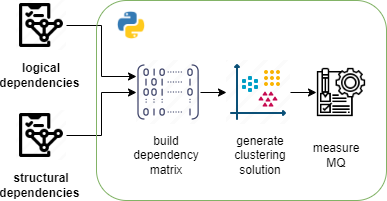
\includegraphics[width=\columnwidth]{clustering-generation.png}
\caption{Clustering solution creation process diagram}
\label{fig:clustering-gen}
\end{figure}

Louvain Clustering is a community detection algorithm designed for finding clusters or communities in complex networks. The Louvain method involves a greedy algorithm that moves nodes between clusters to obtain clusters that are highly interconnected \cite{louvain_clustering}.

\subsection{Evaluation using MQ metric}
The resulting clustering solution is then evaluated using the Modularity Quality (MQ) metric . The MQ metric can vary between -1 and 1, where -1 means no cohesion within the modules, and 1 means no coupling between the modules \cite{mqmetric}.

To compare the clustering solutions and their MQ evaluation, we generated clustering solutions under three different scenarios. The first one by using only structural dependencies, the second one by using only logical dependencies, and the third one by using logical and structural dependencies to populate the dependency matrix that is further used in cluster generation.


\section{Results}
\label{results}


The results of the scenarios mentioned in section \ref{method} are presented in tables \ref{tab:clustering-results1} and \ref{tab:clustering-results2}.
 In both tables, the first row shows the results from the clustering analysis relying solely on structural dependencies (scenario 1, which is used as a baseline for comparison). We highlighted the results of structural dependencies in both tables for a more easy comparison with the results involving also logical dependencies.

Table \ref{tab:clustering-results1} presents the results when using only logical dependencies for software clustering. All rows, except the first one, represent the measurements obtained from logical dependencies extracted with varying strength thresholds.


\begin{table}[htbp]
  \centering
  \caption{Louvain clustering results for LD only vs SD only}
  \label{tab:clustering-results1}
  \begin{tabular}{lc|c|c}
    \toprule
    \textbf{Dataset} & \textbf{Entities} & \textbf{Cluster} & \textbf{MQ } \\
    & \textbf{Count} & \textbf{count} &  \textbf{metric} \\
    \midrule
    SD only & 517 & 14 &  0.085  \\
    \midrule
LD  strength    10\%    &   320 &   75  &   0.383   \\
LD  strength    20\%    &   215 &   53  &   0.547   \\
LD  strength    30\%    &   174 &   44  &   0.558   \\
LD  strength    40\%    &   152 &   40  &   0.58    \\
LD  strength    50\%    &   138 &   35  &   0.604   \\
LD  strength    60\%    &   120 &   34  &   0.587   \\
LD  strength    70\%    &   106 &   32  &   0.577   \\
LD  strength    80\%    &   92  &   29  &   0.576   \\
LD  strength    90\%    &   79  &   24  &   0.606   \\
LD  strength    100\%   &   64  &   19  &   0.611   \\
    \bottomrule
  \end{tabular}
\end{table}


Table \ref{tab:clustering-results2} presents the results when using logical dependencies combined with structural dependencies for software clustering. All rows, except the first one, represent the measurements obtained from logical dependencies extracted with varying strength thresholds combined with structural dependencies extracted from static code analysis.

In both tables, the second column shows the total count of different entities forming dependencies in the system. The thirth column indicates the number of clusters obtained after injecting the dependencies to the Lovian algorithm. Lastly, the forth column indicates the MQ metric result computed for on the obtained clusters.

\begin{table}[htbp]
  \centering
  \caption{Louvain clustering results for LD and SD combined vs SD only}
  \label{tab:clustering-results2}
  \begin{tabular}{lc|c|c}
    \toprule
    \textbf{Dataset} & \textbf{Entities} & \textbf{Cluster} & \textbf{MQ } \\
    & \textbf{Count} & \textbf{count} &  \textbf{metric} \\
    \midrule
    SD only & 517 & 14 &  0.085  \\
    \midrule
SD  LD  strength    10\%    &   517 &   15  &   0.087   \\
SD  LD  strength    20\%    &   517 &   13  &   0.071   \\
SD  LD  strength    30\%    &   517 &   13  &   0.071   \\
SD  LD  strength    40\%    &   517 &   13  &   0.071   \\
SD  LD  strength    50\%    &   517 &   13  &   0.071   \\
SD  LD  strength    60\%    &   517 &   13  &   0.071   \\
SD  LD  strength    70\%    &   517 &   13  &   0.071   \\
SD  LD  strength    80\%    &   517 &   13  &   0.071   \\
SD  LD  strength    90\%    &   517 &   13  &   0.071   \\
SD  LD  strength    100\%   &   517 &   13  &   0.072   \\

    \bottomrule
  \end{tabular}
\end{table}

Can be observed in Table \ref{tab:clustering-results1} that the MQ results for clustering solutions based solely on logical dependencies (LD) are not better than those based solely on structural dependencies (SD). In Column 2, it is noticeable that the total number of entities used decreases as the strength threshold increases. This trend is expected because stricter thresholds filter out more entities. But it is noticeable that this affects the overall quality of the clustering solutions obtained.

In a scenario where structural dependencies aren't accessible for extraction, logical dependencies can be used as a substitute, but with less strict filtering compared to when they're intended to be combined with structural dependencies.


On the other hand, in Table \ref{tab:clustering-results2} can be observed that starting with the strength threshold of 20\% the MQ results for clustering solutions based on logical dependencies (LD) combined with structural dependencies (SD) are better than those based solely on structural dependencies (SD). 


\section{Discussion}
\label{discussion}

Based on the results from table \ref{tab:clustering-results2}, we can observe that the combined approach of structural dependencies and logical dependencies gives a Modularity Quality (MQ) metric of 0.071, which is an improvement over the 0.085 MQ metric obtained when considering only structural dependencies. 

Beyond the positive result indicated by the MQ metric, we searched for further validation by human software engineering expert opinion. After thoroughly studying and understanding the analyzed system source code and documentation, we evaluated the remodularization proposals resulting from the two clustering solutions.

The two clustering solutions compared are the clustering solution obtained only from structural dependencies, in comparison to the clustering solution obtained from using both structural and logical dependencies, filtered with a threshold of 20\% for strength.

The clustering solution relying solely on structural dependencies consists of 14 clusters, while the solution using both structural and logical dependencies consists of 13 clusters, both solutions involve the same number of entities (517). The entities listed below are placed in different clusters: 


\begin{itemize}
    \item taskdefs.Available\$FileDir
    \item taskdefs.Concat and its inner classes taskdefs.Concat\$1, taskdefs.Concat\$ MultiReader, taskdefs.Concat\$ TextElement
    \item taskdefs.Javadoc\$AccessType
    \item util.WeakishReference and its inner class util.WeakishReference\$HardReference
    \item taskdefs.Replace and its inner classes taskdefs.Replace\$ NestedString, taskdefs.Replace\$ Replacefilter
\end{itemize}

The migration of entities between clusters is ilustared in Figure \ref{fig:clustersmigration}. Given that the inner classes are shifted from one cluster to another in identical way as the outer class, we omitted the inner classes from the diagram.

As the cluster number itself is not significant and may vary across different script runs (labels might vary), we will refer to each individual cluster resulting from structural dependencies as \textit{Cluster A} and to the ones resulting from both logical and structural dependencies as \textit{Cluster B}.

\begin{figure}
\centering
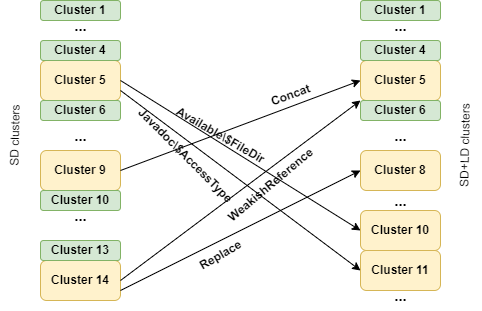
\includegraphics[width=\columnwidth]{clusters.png}
\caption{Migration of entities between clusters}
\label{fig:clustersmigration}
\centering
\end{figure}

\subsection{taskdefs.Concat and its inner classes}

To  have a better overview into how and why entities are transferred between clusters, we depicted Concat's logical and structural connections in Figure \ref{fig:dep_concat}. Additionally, Figure \ref{fig:clusterAconcat} illustrates connections within Cluster A, while Figure \ref{fig:clusterBconcat} does the same for Cluster B.

In Cluster A, the Concat class and its inner classes (Concat\$1, Concat\$MultiReader, Concat\$TextElement) are placed together with conditions like Available, And, Or, IsTrue, Equals, IsReference, Contains.

On the other hand, in Cluster B are placed with classes associated with file manipulation and archive operations such as Ear, Jar, War, and Zip, as well as utility classes for file handling like FileUtils and JavaEnvUtils, and entities for zip file processing (ZipEntry, ZipFile).  This placement is due to the logical dependencies that Concat class has with FileUtils and FileSet in the versioning system.

To assess whether the placement of Concat in Cluster B is better then in Cluster A, we referred to the official Ant documentation. According to the documentation: "This class contains the 'concat' task, used to concatenate a series of files into a single stream" \cite{ant_concat}. Therefore, judging by its usage and purpose according to the documentation, positioning the Concat class along with its inner classes in Cluster B is more suitable than in Cluster A.


\begin{figure}
\centering
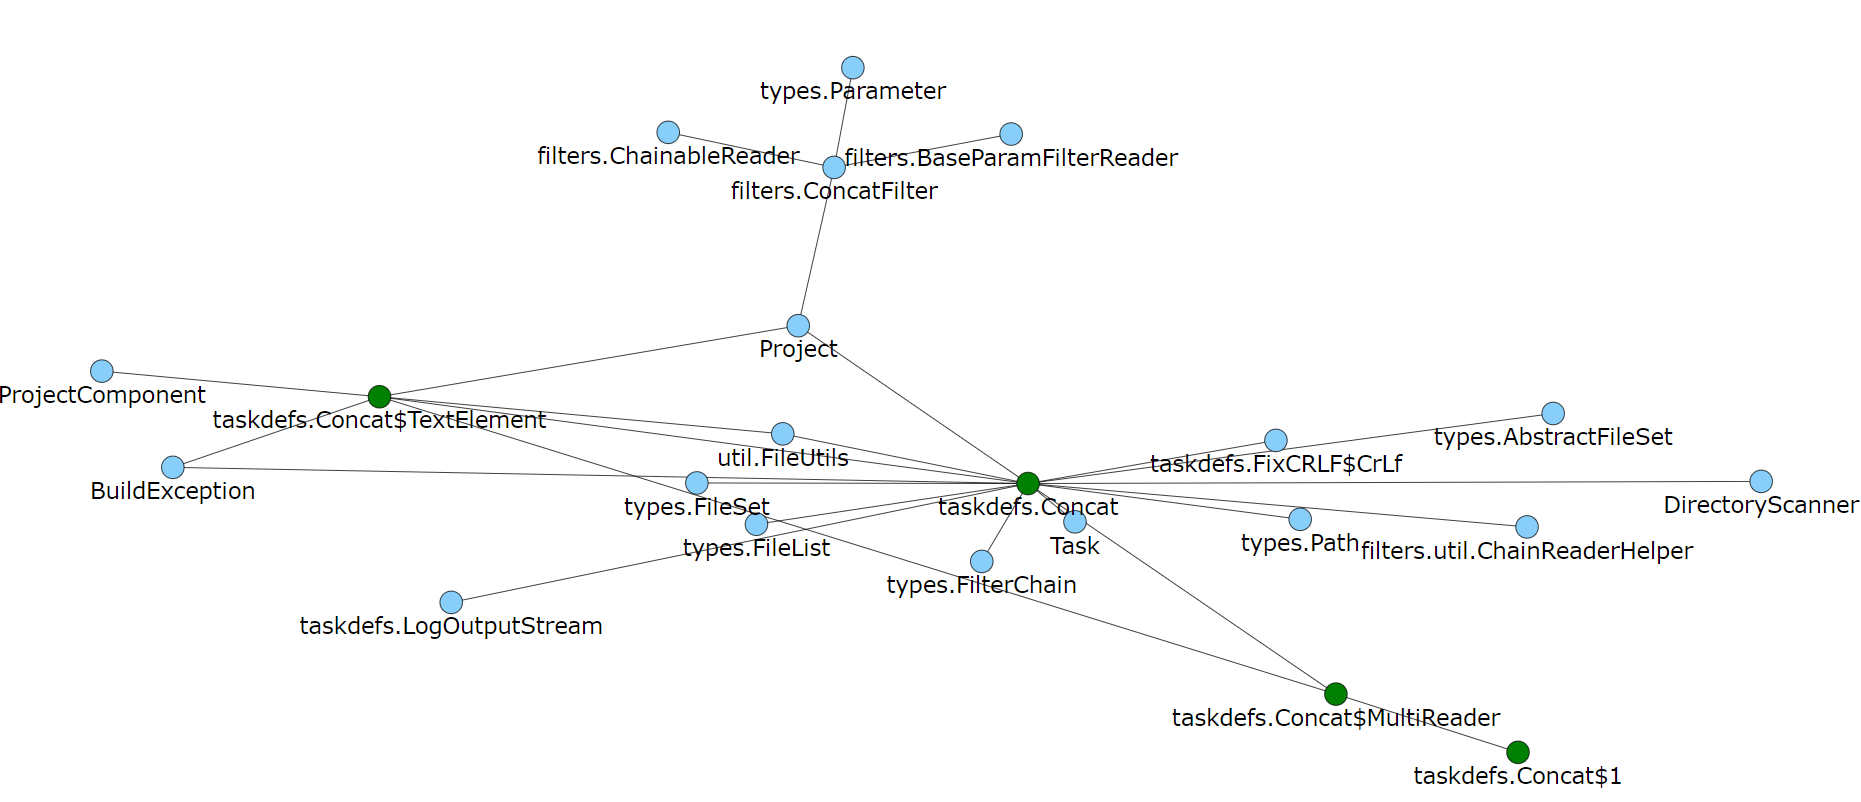
\includegraphics[width=\columnwidth]{dep_concat.png}
\caption{Dependencies (LD and SD) of Concat class}
\label{fig:dep_concat}
\centering
\end{figure}


\begin{figure}
\centering
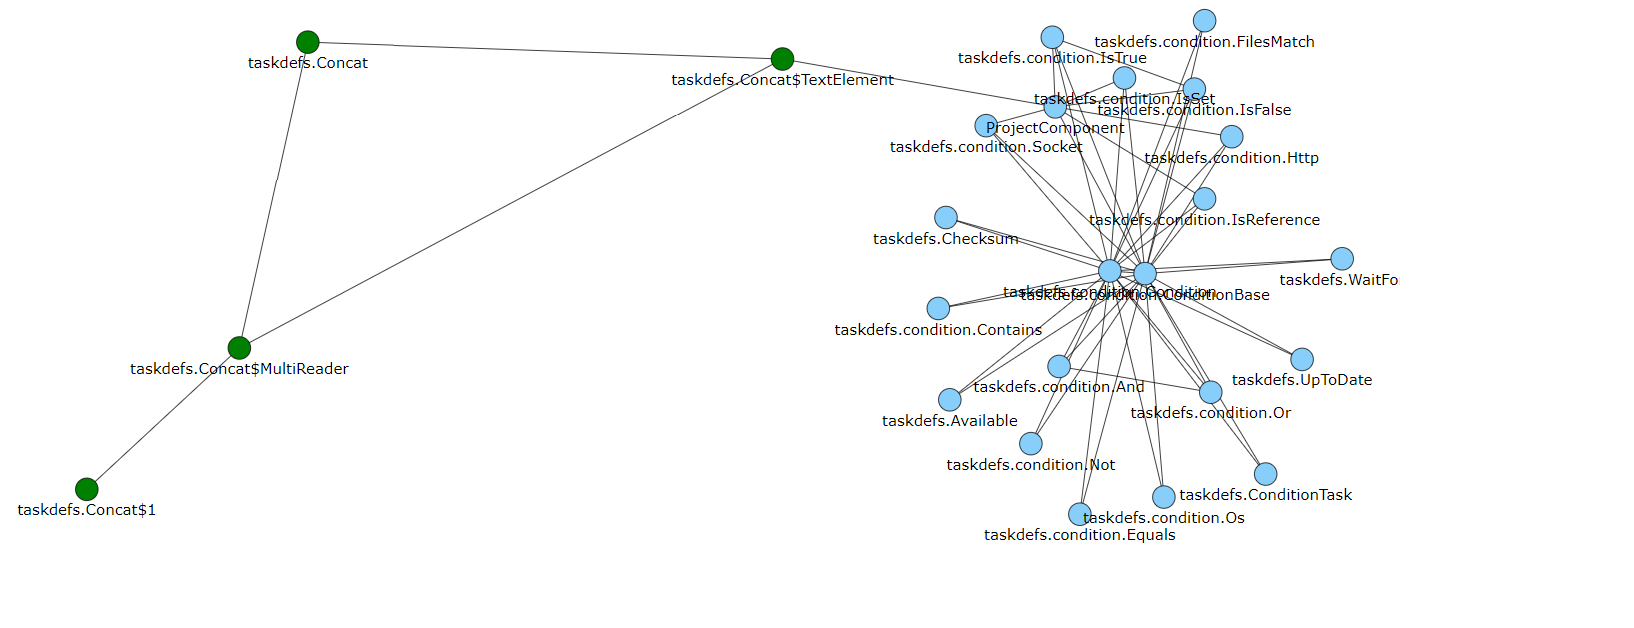
\includegraphics[width=\columnwidth]{cluster_concatSD.PNG}
\caption{Placement of Concat in ClusterA (SD); cluster size: 25}
\label{fig:clusterAconcat}
\centering
\end{figure}


\begin{figure}
\centering
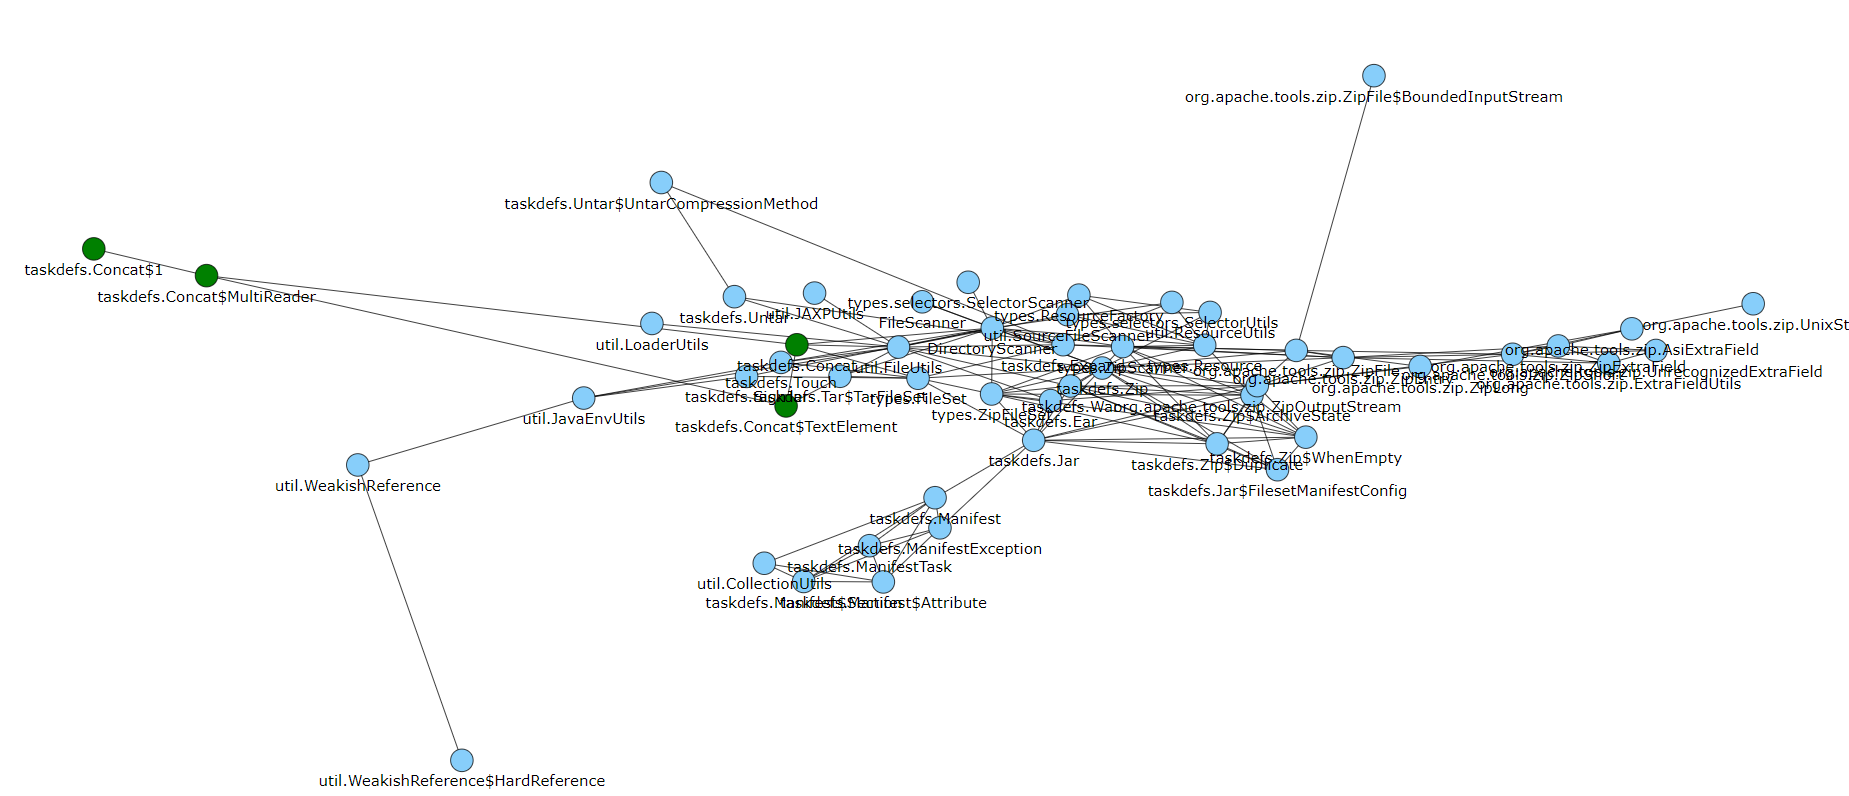
\includegraphics[width=\columnwidth]{cluster_concatSDLD.PNG}
\caption{Placement of Concat in ClusterB (SD and LD); cluster size: 52}
\label{fig:clusterBconcat}
\centering
\end{figure}

\subsection{taskdefs.Available\$FileDir}

In Cluster A the entity 'taskdefs.Available\$FileDir' is in the same cluster with entities that are related to the build process (ProjectHelper, TaskAdapter, ComponentHelper), but not with entities that have any relation to condition checks or file existence evaluations or with its outer class. 

Cluster B contains entities that are related to condition checking (And, Contains, Equals, Or, UpToDate), and also with the outer class of 'taskdefs.Available\$FileDir',  'taskdefs.Available'. The movement of entities from Cluster A to Cluster B was influenced by the logical dependencies between 'taskdefs.Available' and 'taskdefs.Available\$FileDir'.

The documentation description for 'taskdefs.Available' states: "Will set the given property if the requested resource is available at runtime. This task may also be used as a condition by the condition task."\cite{ant_concat}.
This reinforces its placement in Cluster B, which is centered around task definitions and conditions related to build processes.



\subsection{ taskdefs.Replace and its inner classes}

\begin{figure}
\centering
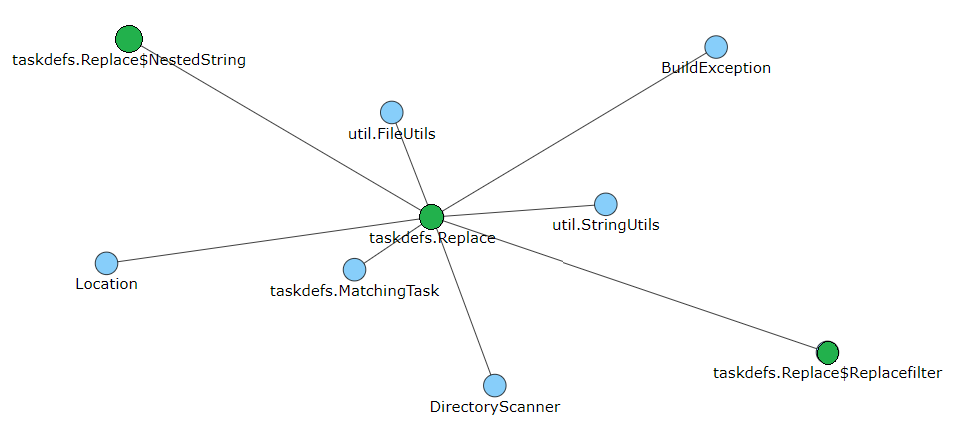
\includegraphics[width=\columnwidth]{dep_replace.png}
\caption{Ant dependencies (LD and SD) of Replace and its inner classes}
\label{fig:dep_replace}
\centering
\end{figure}

\begin{figure}
\centering
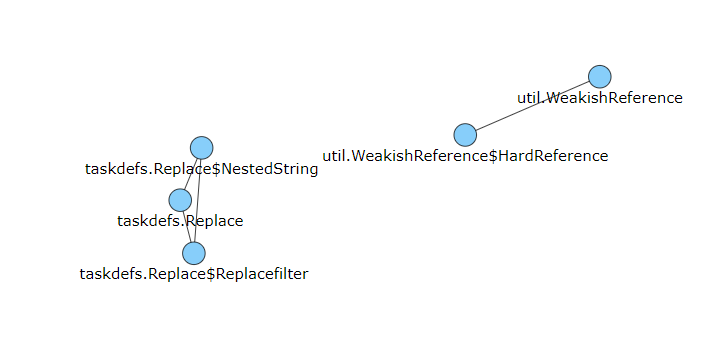
\includegraphics[width=\columnwidth]{cluster_replaceSD.PNG}
\caption{Placement of Replace in ClusterA (SD); cluster size: 5}
\label{fig:clusterAreplace}
\centering
\end{figure}


\begin{figure}
\centering
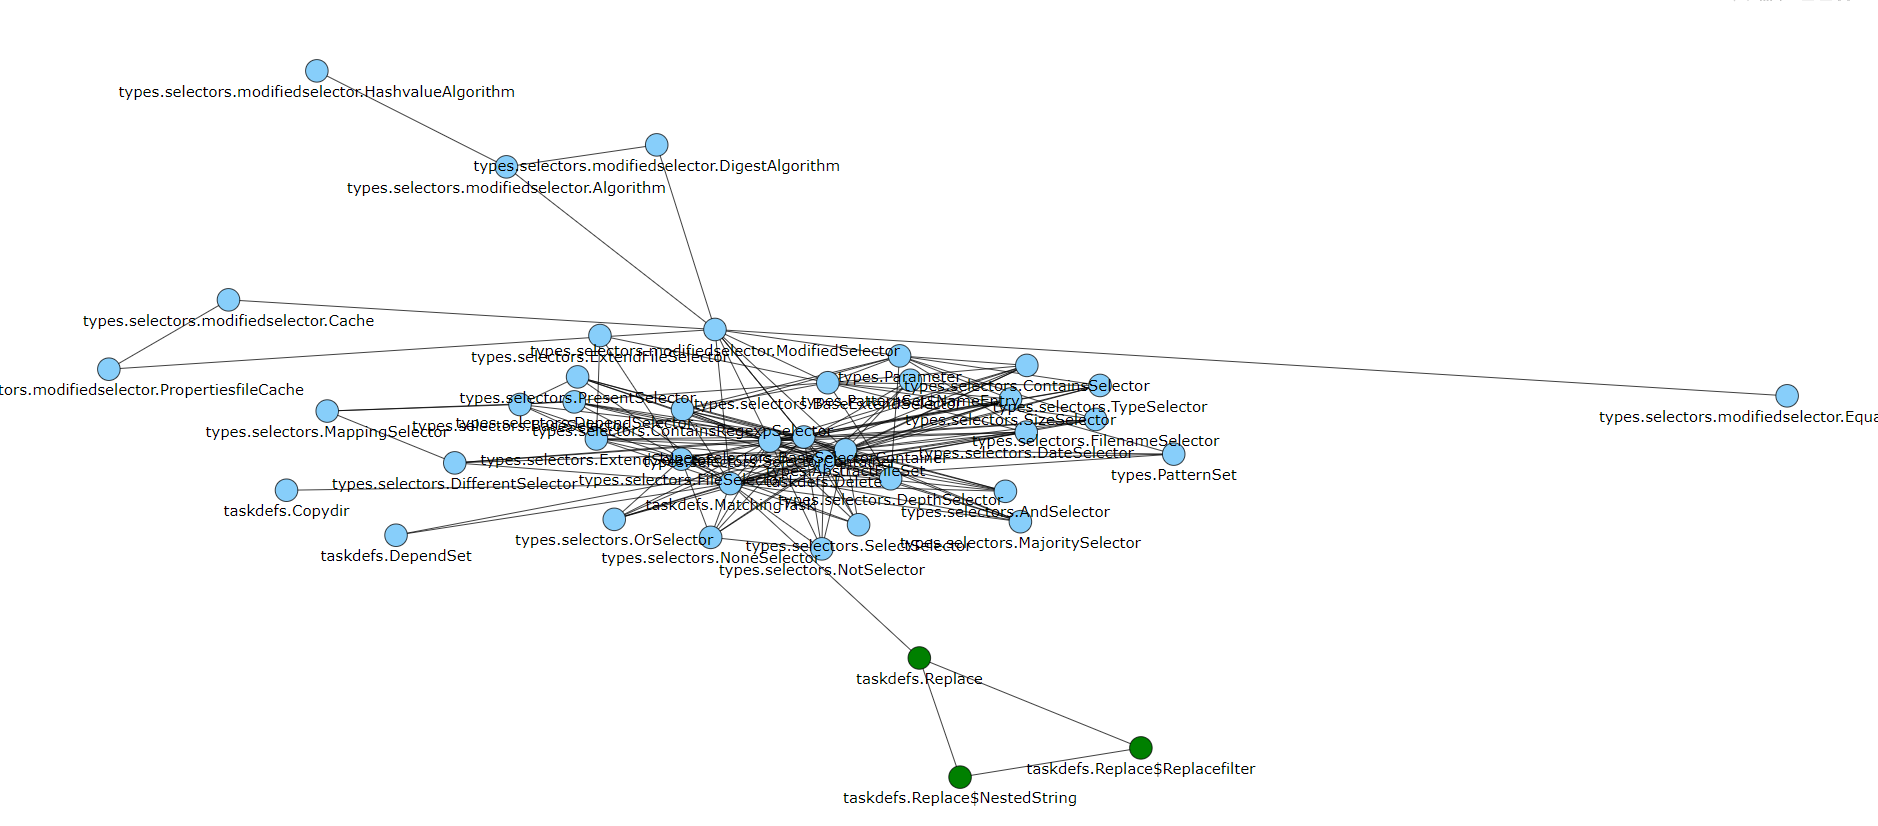
\includegraphics[width=\columnwidth]{cluster_replaceSDLD.PNG}
\caption{Placement of Replace in ClusterB (SD and LD); cluster size: 42}
\label{fig:clusterBreplace}
\centering
\end{figure}


We depicted the logical and structural connections of Replace in Figure \ref{fig:dep_replace}. Figure \ref{fig:clusterAreplace} illustrates connections within Cluster A, while Figure \ref{fig:clusterBreplace} does the same for Cluster B.

Replace and its inner classes are placed in Cluster B with entities with which they share common functionality and purpose, such as Copydir, Delete, DependSet, or MatchingTask. These entities are involved in similar tasks and operations. On the other hand, the placement in Cluster A, with WeakishReference and its inner class doesn't seem good, as these entities are completly unrelated.  

The movement of entities from Cluster A to Cluster B was influenced by the strong logical dependency between 'taskdefs.Replace' and 'taskdefs.MatchingTask'.


Also, the cluster from figure \ref{fig:clusterAreplace} is the 14th cluster that is missing from the clustering solution based on logical and structural dependencies. We obtained 14 clusters from structural dependecies only and 13 from logical combined with structural dependencies. This particular cluster is essentially comprised of two unrelated entities: Replace and WeakishReference. Due to their logical dependencies, both entities are grouped within larger clusters that share similar functionalities in the SD and LD solution.



\section{Conclusion and Future work}
\label{conclusion}

Based the outcomes from Section \ref{results} and the analysis from Section \ref{discussion}, it is clear that incorporating logical dependencies improves the quality of clustering solutions. 
This reinforces the idea that dependencies extracted from the versioning system contribute with new information that isn't otherwise available through code analysis.  Our current findings are that using logical dependencies combined with structural dependencies improves the quality of the software clustering solution. Using only logical dependencies as input for software clustering does not attain the same quality as with structural dependencies, but it could be an alternative solution if the analysis of the source code is not possible.

In our forthcoming work, we intend to expand the project list for our software clustering analysis to better understand the effectiveness of integrating both structural and logical dependencies. Additionally, we'll explore alternative metrics besides MQ to validate the improved quality of these solutions compared to those based solely on structural dependencies.

\bibliographystyle{IEEEtran}
\bibliography{logicaldepd}

\end{document}
